%% Nothing to modify here.
%% make sure to include this before anything else

\documentclass[10pt]{beamer}
\usetheme{Szeged}

% packages
\usepackage{color}
\usepackage{listings}

% color definitions
\definecolor{mygreen}{rgb}{0,0.6,0}
\definecolor{mygray}{rgb}{0.5,0.5,0.5}
\definecolor{mymauve}{rgb}{0.58,0,0.82}

% re-format the title frame page
\makeatletter
\def\supertitle#1{\gdef\@supertitle{#1}}%
\setbeamertemplate{title page}
{
  \vbox{}
  \vfill
  \begin{centering}
  \begin{beamercolorbox}[sep=8pt,center]{title}
      \usebeamerfont{supertitle}\@supertitle
   \end{beamercolorbox}
    \begin{beamercolorbox}[sep=8pt,center]{title}
      \usebeamerfont{title}\inserttitle\par%
      \ifx\insertsubtitle\@empty%
      \else%
        \vskip0.25em%
        {\usebeamerfont{subtitle}\usebeamercolor[fg]{subtitle}\insertsubtitle\par}%
      \fi%     
    \end{beamercolorbox}%
    \vskip1em\par
    \begin{beamercolorbox}[sep=8pt,center]{author}
      \usebeamerfont{author}\insertauthor
    \end{beamercolorbox}
    \begin{beamercolorbox}[sep=8pt,center]{institute}
      \usebeamerfont{institute}\insertinstitute
    \end{beamercolorbox}
    \begin{beamercolorbox}[sep=8pt,center]{date}
      \usebeamerfont{date}\insertdate
    \end{beamercolorbox}\vskip0.5em
    {\usebeamercolor[fg]{titlegraphic}\inserttitlegraphic\par}
  \end{centering}
  \vfill
}
\makeatother

% insert frame number
\expandafter\def\expandafter\insertshorttitle\expandafter{%
      \insertshorttitle\hfill%
\insertframenumber\,/\,\inserttotalframenumber}

% preset-listing options
\lstset{
  backgroundcolor=\color{white},   
  % choose the background color; 
  % you must add \usepackage{color} or \usepackage{xcolor}
  basicstyle=\footnotesize,        
  % the size of the fonts that are used for the code
  breakatwhitespace=false,         
  % sets if automatic breaks should only happen at whitespace
  breaklines=true,                 % sets automatic line breaking
  captionpos=b,                    % sets the caption-position to bottom
  commentstyle=\color{mygreen},    % comment style
  % deletekeywords={...},            
  % if you want to delete keywords from the given language
  extendedchars=true,              
  % lets you use non-ASCII characters; 
  % for 8-bits encodings only, does not work with UTF-8
  frame=single,                    % adds a frame around the code
  keepspaces=true,                 
  % keeps spaces in text, 
  % useful for keeping indentation of code 
  % (possibly needs columns=flexible)
  keywordstyle=\color{blue},       % keyword style
  % morekeywords={*,...},            
  % if you want to add more keywords to the set
  numbers=left,                    
  % where to put the line-numbers; possible values are (none, left, right)
  numbersep=5pt,                   
  % how far the line-numbers are from the code
  numberstyle=\tiny\color{mygray}, 
  % the style that is used for the line-numbers
  rulecolor=\color{black},         
  % if not set, the frame-color may be changed on line-breaks 
  % within not-black text (e.g. comments (green here))
  stepnumber=1,                    
  % the step between two line-numbers. 
  % If it's 1, each line will be numbered
  stringstyle=\color{mymauve},     % string literal style
  tabsize=4,                       % sets default tabsize to 4 spaces
  title=\lstname                   
  % show the filename of files included with \lstinputlisting; 
  % also try caption instead of title
}

% macro for code inclusion
\newcommand{\includecode}[2][c]{
	\lstinputlisting[caption=#2, style=custom#1]{#2}
}	% nothing to do here
\usepackage[english]{babel}

\usepackage[utf8]{inputenc}

\newcommand{\course}{
	C introduction
}

\author{
	Richard Mörbitz,
	Manuel Thieme
}

\lstset{
	language = C,
	showspaces = false,
	showtabs = false,
	showstringspaces = false,
	tabsize = 4,
	escapechar = @
} % TODO modify this if you have not already done so

% meta-information
\usepackage{tikz}

\newcommand{\topic}{
    Basic program structure
}

\definecolor{orange}{RGB}{255,127,0}

% nothing to do here
\title{\topic}
\supertitle{\course}
\date{}

% the actual document
\begin{document}

\maketitle

\begin{frame}{Contents}
	\tableofcontents
\end{frame}

\section{Setup}
\subsection{}
\begin{frame}{OS's you may use}
	\begin{columns}[T]
		\column{.3\textwidth}
		\centering
		\only<1>{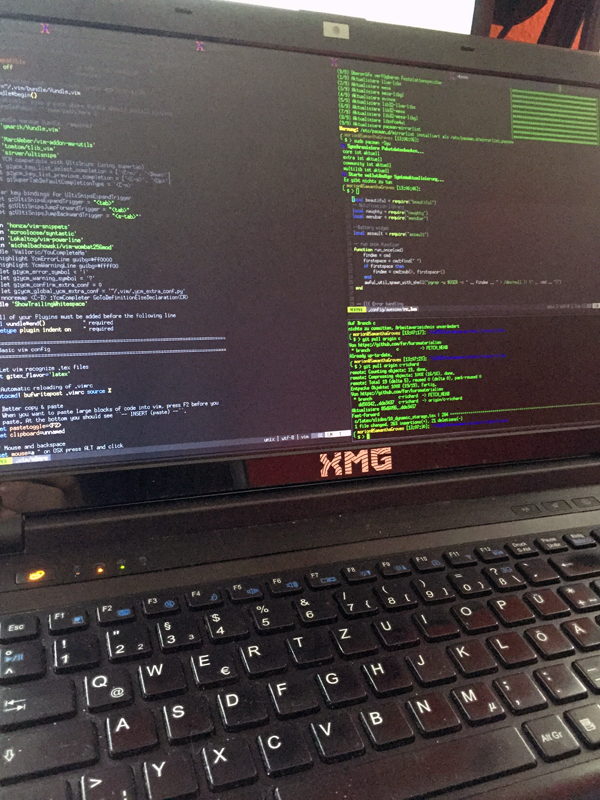
\includegraphics[scale=.15]{../img/Linux.JPG}\\}
		\only<2->{
\includegraphics[scale=.15]{../img/ArchLinux.JPG}\\}
		Linux\\
		\uncover<2->{\textcolor{green}{recommended}}
		\column{.3\textwidth}
		\centering
		\only<1-2>{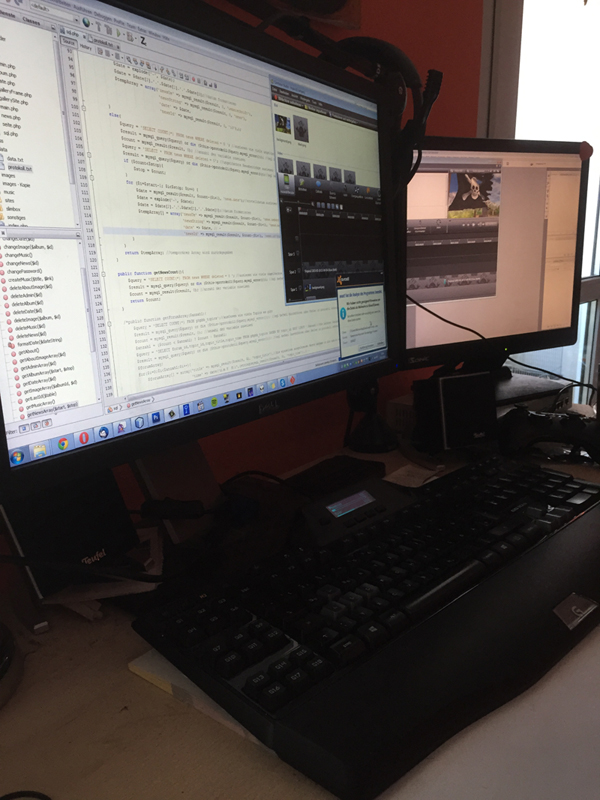
\includegraphics[scale=.15]{../img/Windows.JPG}\\}
		\only<3->{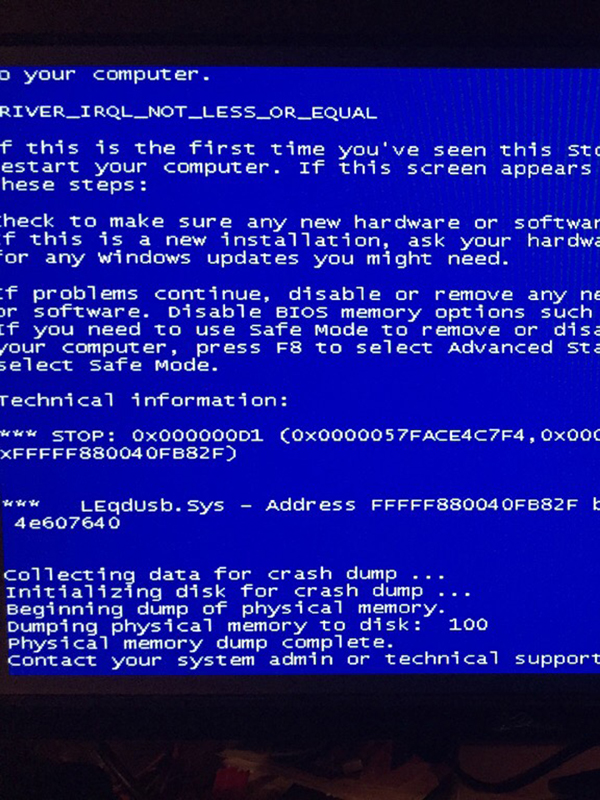
\includegraphics[scale=.15]{../img/Windows8.JPG}\\}
		Windows\\
		\uncover<3->{\textcolor{orange}{supported}}
		\column{.3\textwidth}
		\centering
		\only<1-3>{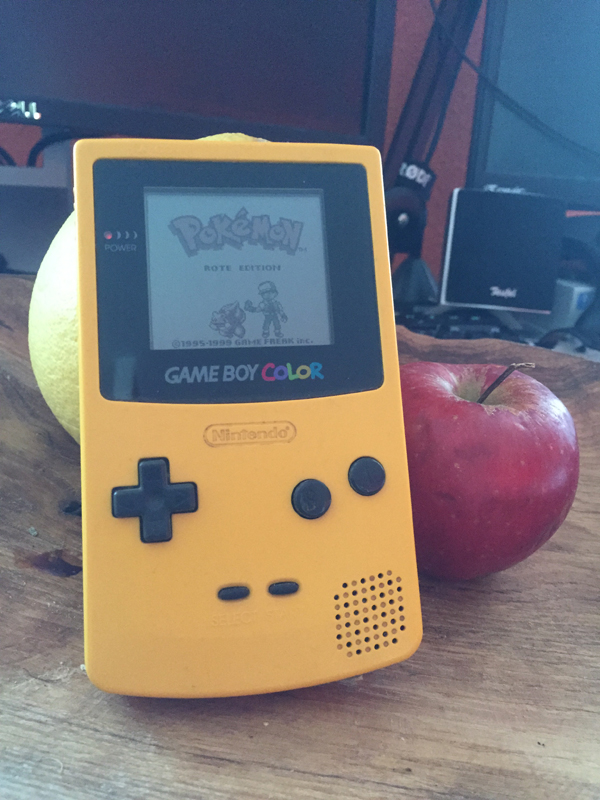
\includegraphics[scale=.15]{../img/iOS.JPG}\\}
		\only<4->{
\includegraphics[scale=.15]{../img/iOSX.JPG}\\}
		\begin{tikzpicture}
			\node at (0,0) {Mac OS};
			\begin{uncoverenv}<1-3>
				\node at (.88,0) {X};
			\end{uncoverenv}
			\begin{uncoverenv}<4->
				\draw[thick,red] (-.6,.13) -- (.6,-.13);
				\draw[thick,red] (-.6,-.13) -- (.6,.13);
			\end{uncoverenv}
		\end{tikzpicture}
	\end{columns}
\end{frame}
\begin{frame}[fragile]{Installing gcc on Linux}
	Ubuntu / Debian: 
	\begin{lstlisting}[numbers=none]
$ sudo apt-get install gcc
\end{lstlisting} \ \\ \ \\
	Arch:
	\begin{lstlisting}[numbers=none]
$ sudo pacman -S gcc
\end{lstlisting} \ \\ \ \\
	... and you're done ;-)
\end{frame}
\begin{frame}{cygwin}
	\begin{itemize}
		\item Download installer from \textit{https://cygwin.com/install.html}
		\item Run it
		\begin{itemize}
			\item "Install from Internet"
			\item Choose your installation path
			\item Choose path for installation files
			\item "Direct Connection"
			\item Choose a mirror
			\item Important software already is selected
			\item \textbf{Optional}: powerful editor "vim" in \textit{Editors}
			\item \textbf{Recommended}: "GDB" in \textit{Devel} and "libncurses-devel" in \textit{libs} for the advanced course
			\item Watching loading bars...
			\item ???
			\item Profit!
		\end{itemize}
		\item Use cygwin-console like a linux terminal
	\end{itemize}
\end{frame}
\section{Hello World!}
\subsection{}
\begin{frame}[fragile]{The first program}
	\begin{itemize}
		\item Create a new file named \textbf{main.c}.
		\item Open it in your text editor of trust.
		\item Fill it as follows:
	\end{itemize}
	\begin{lstlisting}
#include <stdio.h>

int main(int argc, char *argv[]) {
	printf("Hello World!\n");
	/* Print "Hello World!" on the
	   command line */
	return 0;
}
\end{lstlisting}
\end{frame}
\begin{frame}[fragile]{From source to bits}
	\centering
	Source code\\\ \\
	$\Downarrow$\\\ \\
	\begin{lstlisting}[numbers=none]
$ gcc main.c
\end{lstlisting}
(Preprocessing, compiling, assembling, linking)
	\ \\\ \\
	$\Downarrow$\\\ \\
	Executable program\\\ \\
	\begin{columns}[T]
		\column{.3\textwidth}
		Linux (\textbf{a.out})
		\begin{lstlisting}[numbers=none]
$ ./a.out
\end{lstlisting}
		\column{.3\textwidth}
		Windows (\textbf{a.exe})
		\begin{lstlisting}[numbers=none]
$ ./a.exe
\end{lstlisting}
	\end{columns}
\end{frame}
\section{Program structure}
\subsection{}
\begin{frame}[fragile]{A basic program}
	\begin{columns}[T]
		\column{.6\textwidth}
		\begin{lstlisting}
#include <stdio.h>

int main(int argc, char *argv[]) {

	printf("Hello World!\n");
	/* Print "Hello World!" on the
	   command line */

	return 0;
}
\end{lstlisting}
		\column{.4\textwidth}
		
		\ \\$\left. \begin{array}{c}\\\end{array}\right\rbrace $ Preprocessor statements
		\ \\\ \\$\left. \begin{array}{c}\\\\\\\\\\\\\end{array}\right\rbrace $ Main function
	\end{columns}
\end{frame}
\begin{frame}[fragile]{Preprocessor statements}	
	\begin{itemize}
		\item Processed before compilation
		\item Have their own language, start with a \textit{\#}
	\end{itemize}
	\begin{lstlisting}
#include <stdio.h>
\end{lstlisting}
	\begin{itemize}
		\item Includes the \textbf{standard input/output library} (needed for printf, which is defined there) \\ \ \\
		\item Can also be used to define constants and much more, e.g.
	\end{itemize}
\begin{lstlisting}[numbers=none]
#define THE_ANSWER 42
\end{lstlisting}
\end{frame}
\begin{frame}[fragile]{The main function}
	\begin{itemize}
		\item Basic function
		\item Exists \textbf{exactly once} per program
		\item Called on program start
	\end{itemize}
	\StartLineAt{3}
	\begin{lstlisting}
int main(int argc, char *argv[]) {
\end{lstlisting}
	\begin{itemize}
		\item As a function, \textit{main()} takes parameters
		\item Get used to \textit{argc} and \textit{argv}, they will be explained later
		\item '$\lbrace$' marks the start of the main function scope
	\end{itemize}
\end{frame}
\begin{frame}[fragile]{The main function scope}
	\begin{itemize}
		\item Contains all program statements
		\item They are processed from top to bottom
	\end{itemize} \ \\
	\ \\
	\StartLineAt{9}
	\begin{lstlisting}
	return 0;
}
\end{lstlisting}
	\begin{itemize}
		\item Last statement, ends main function (and thus the whole program)
		\item \textit{0} tells the OS that everything went right
		\item '$\rbrace$' marks the end of the main function scope
	\end{itemize}
\end{frame}
\begin{frame}[fragile]{Statements}
	\begin{itemize}
		\item Instructions for the computer
		\item End with a \textit{;} (semicolon)
	\end{itemize}
	\StartLineAt{5}
	\begin{lstlisting}
	printf("Hello World!\n");
\end{lstlisting} \ \\ \ \\
	\begin{itemize}
		\item There is the empty statement:
	\end{itemize}
	\begin{lstlisting}[numbers=none]
	;
\end{lstlisting}
	\begin{itemize}
		\item All statements are located in function blocks
	\end{itemize}
\end{frame}
\begin{frame}[fragile]{Comments}
	\begin{itemize}
		\item Information for the programmer, cut out before compilation
	\end{itemize}
	Single line comments:
	\StartLineAt{6}
	\begin{lstlisting}
	// Print "Hello World!" on the command line
\end{lstlisting}
	Block comments (mutli-line):
	\StartLineAt{6}
	\begin{lstlisting}
	/* Print "Hello World!"
	   on the command line */
\end{lstlisting}
	Better use of block comments:
	\StartLineAt{6}
	\begin{lstlisting}
	/*
	 * Print "Hello World!"
	 * on the command line
	 */
\end{lstlisting}
\end{frame}
\section{Style}
\subsection{}
\begin{frame}[fragile]{A few words on style}
	\begin{itemize}
		\item There can be multiple statements on one line
		\item Intendation is not nessessary at all
		\item<2-> \textbf{But}...
	\end{itemize}
	\ \\
	\begin{uncoverenv}<2->
	\begin{lstlisting}[numbers=none]
#include <stdio.h>
int
main	(int argc, char *argv[]){printf("Hello World!\n");
		// Prints
/*"Hello World!"			*/
		return 0;}
\end{lstlisting}
	\end{uncoverenv}
\end{frame}
\begin{frame}{Much more enjoyable}
	\begin{itemize}
		\item Put each statement on a single line
		\item Intend every statement in the main function by one tab / 4 \textit{spaces}
		\item Use \textit{/* ... */} rather than \textit{// ...}
		\item Write the main function arguments directly behind \textit{main}
		\item Leave a \textit{space} between the closing ')' and the opening '\{'
	\end{itemize}
\end{frame}


% nothing to do from here on
\end{document}
